\documentclass{beamer}

\usepackage{default}

\usetheme{Malmoe}
\usecolortheme{dolphin}

\title{Extensions on Contract Net Protocol for AGVs}
\subtitle{Multi-Agent Systems}

\author{Jens Claes \and Victor Le Pochat}
\date{June 6, 2016}

\begin{document}
	\frame{\titlepage}

	\section{Introduction}
	
	\begin{frame}{Objectives \& Hypotheses}
		\begin{itemize}
		\item CNET vs CNCP vs DynCNET
		\item Hypotheses:
			\begin{itemize}
			\item Compare
				\begin{itemize}
				\item Profit
				\item Delivery time
				\item \# clients undelivered
				\item Message count
				\end{itemize}
			\item Influence on profit
				\begin{itemize}
				\item \# Drones
				\item \# Warehouses
				\item \# Clients
				\end{itemize}
			\end{itemize}
		\end{itemize}
	\end{frame}
	\note{Hypotheses zelf gewoon zeggen}
		
	\begin{frame}{Setting}
		\begin{itemize}
		\item Package delivery company
		\item Drones (UAV)
		\item Battery-constrained
		\item Warehouses
		\item 2 types clients
		\item Fines
		\end{itemize}
	\end{frame}

	\section{Theory}
	
	\begin{frame}{Contract Net Protocol (CNET)}
		\begin{itemize}
			\item Assigning tasks to (idle) agents
			\item Distributed manner
			\item Contract negotiation between manager and contractor
			\begin{itemize}
				\item M: Task announcement
				\item C: Bid
				\item M: Awarding
				\item C: Execution
			\end{itemize}
		\end{itemize}
	\end{frame}
	
	\begin{frame}{Contract Net Protocol (CNET)}
	  \begin{columns}[T] % the "c" option specifies center vertical alignment
	  \column{.5\textwidth} % column designated by a command
	   Negotiation protocol
	  \column{.5\textwidth}
	   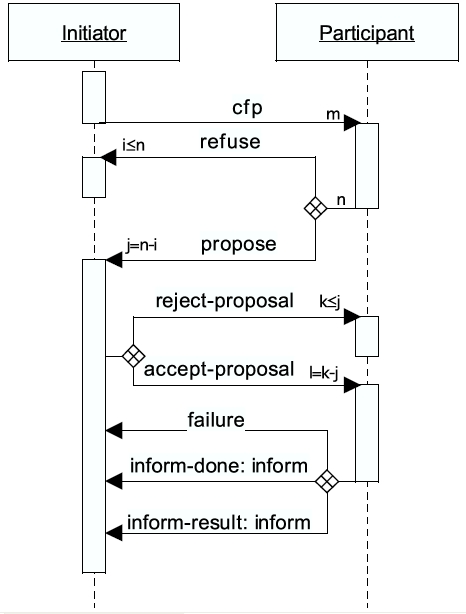
\includegraphics[width=\columnwidth]{FIPA-CNET}
	  \end{columns}
	\end{frame}

	\begin{frame}{Contract Net with Confirmation (CNCP)}
		\begin{itemize}
			\item CNET problem: early commitment
			\item CNCP solution: full commitment when awarded
			\item Contractor submits bid but continues bidding
			\item When awarded, first check if contractor accepts
			\begin{itemize}
				\item if yes: award \& execute task
				\item if no: try next best contractor
			\end{itemize}
		\end{itemize}
	\end{frame}

	\begin{frame}{Dynamic Contract Net (DynCNET)}
		\begin{itemize}
			\item CNET problem: no dynamism
			\item DynCNET solution: allow contract switching
			\item When awarded but still in preparation
			\item Contract final when preparation is finished
		\end{itemize}
	\end{frame}
	
		
	\section{Design}
	\begin{frame}{MAS design}
		\begin{itemize}
			\item Clients have an order
			\item Drone takes up order
			\item Drone collects package at warehouse
			\item Drone flies to client and delivers package
		\end{itemize}
	\end{frame}
	
	\begin{frame}{MAS design}
		\begin{itemize}
			\item Goal: maximize profit
			\begin{itemize}
				\item Allocate task to most suitable drone
				\item Find cheapest warehouse
				\item Minimize crashes
				\begin{itemize}
					\item Keep battery charged
					\item Poisson distribution
				\end{itemize}
				\item Deliver on time
			\end{itemize}
		\end{itemize}
	\end{frame}
	
	\begin{frame}{MAS design comparison}
		\begin{itemize}
			\item Simplified task announcement: only order
			\item CNET: committed to bids
			\item Extension to delay announcement
			\item CNCP: reannounce task instead of trying next best bidder
			\note{omvat ook mergen task acceptance in 1 bericht}
			\item DynCNET: no consideration for oscillation
		\end{itemize}
	\end{frame}
	
	\section{Experiments}
	\begin{frame}{Experiments}
		\begin{itemize}
			\item
		\end{itemize}
	\end{frame}
	
	\section{Conclusion}
	\begin{frame}{Conclusion}
		\begin{itemize}
			\item
		\end{itemize}
	\end{frame}
	
\end{document}
